\documentclass{article}
\usepackage[utf8]{inputenc}
\usepackage{graphicx}
\usepackage{wrapfig}
\usepackage[T1]{fontenc}
\usepackage{amssymb}
\usepackage{siunitx}

\title{Time Constant of a Capacitor and Step Response
in RLC Circuits\\ ELP100\\Lab Report 3}
\author{Aditya Agrawal\\2021AM10198\\GROUP 29}
\date{May 4, 2022}

\begin{document}

\maketitle
\tableofcontents
\newpage

\section{ Time Constant in RC Circuit}
\subsection{Aim}
To observe and trace the complete response to step input and to determine the time constant and check with the theoretically calculated value.

\subsection{Apparatus}
\begin{enumerate}
    \item Variable resistor and Multimeter
    \item Function Generator (0 – 3 MHz)
    \item Breadboard and Jumpers
    \item Capacitor of capacitance – 0.22 µF
    \item Digital Storage Oscilloscope (DSO1052B)
\end{enumerate}

\subsection{Theory}
\begin{wrapfigure}{R}{0.2\textwidth}
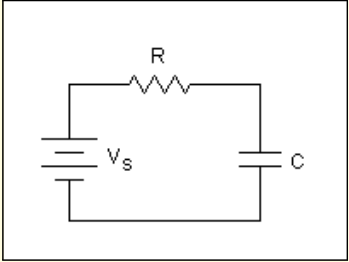
\includegraphics[width=0.2\textwidth]{i1.png}
\end{wrapfigure}
To determine the total response of an RC Series Circuit, we add the zero input response (Natural Response) and the zero state response (Forced Response).
\begin{equation}
    C \frac{dV_{C}}{dt} + \frac{V_{C}}{R} = 0
\end{equation}
In case of Charging, the solution is $V_{C}$ = $V_{0}$(1 − $e^{- \frac{Rt}{L}}$), where RC is known as Time Constant. \\
In case of Discharging, the solution is $V_{C}$ = $V_{0}$$e^{- \frac{Rt}{L}}$, where RC is known as Time Constant.

\subsection{Breadboard Setup}
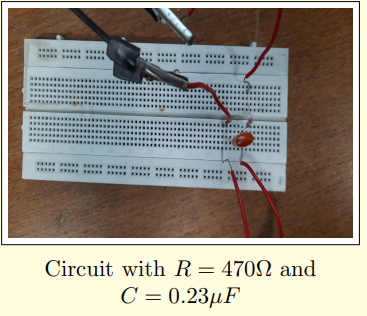
\includegraphics[width=0.5\textwidth]{i2.png}
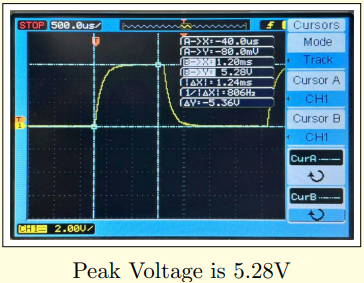
\includegraphics[width=0.55\textwidth]{i3.png}

\subsection{Observation}
\begin{center}
\begin{tabular}{|c|c|c|}
\hline
    Status & Voltage(V) & Time Constant(\tau) \\
    \hline
    Charging & 63\% of 5.28 = 3.33 & 132µs \\
    Discharging & 37\% of 5.28 = 1.94 & 134µs \\
\hline
\end{tabular} \\
\end{center}
\\
\\
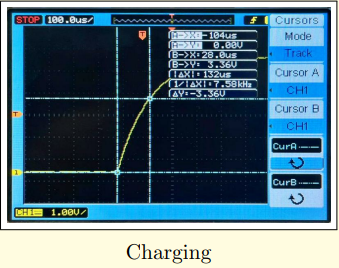
\includegraphics[width=0.6\textwidth]{i4.png}
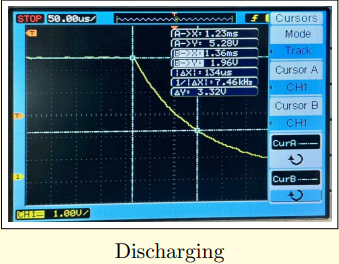
\includegraphics[width=0.6\textwidth]{i5.png}

\subsection{Calculation}
Theoretical Time Constant ($\tau$) = R × C = 470 × 0.23 × $10^{-6}$s=108.1 µs.\\
Calculated Time Constant \approx \SI{133}{\micro\second}

\subsection{Error Analysis}
Error= 133µs - 108.1µs = 24.9 µs\\
Percentage Error= $\frac{24.9}{133}$ × 100 = 18.7\%

\subsection{Conclusion}
Consequently, we were able to measure, within experimental error, the time constant of the series RC circuit using a DSO instrument.
\newpage
\section{Step Response in RLC Circuit}
\subsection{Aim}
To observe and trace the complete response to step input in RLC Circuit.
 \subsection{Apparatus}
 \begin{enumerate}
    \item Variable resistor and Multimeter
    \item Function Generator (0 – 3 MHz)
    \item Breadboard and Jumpers
    \item Capacitor of capacitance – 0.22 µF and Inductance of 2H
    \item Digital Storage Oscilloscope (DSO1052B)
\end{enumerate}
\subsection{Theory}
The general Solution of Voltage in Series RLC Circuit is of the form:\\
\begin{center}
    V(t)=$A_{1}$$e^{-s_{1}t}$ + $A_{2}$$e^{-s_{2}t}$
\end{center}
where $s_{1}$ and $s_{2}$ are solutions of the quadratic equation:\\
\begin{center}
    $s^{2}$ + 2$\alpha$s + $\omega_{0}^{2}$ = 0, where $\alpha$ = $\frac{R}{2L}$ and $\omega_{0}^{2}$=$\frac{1}{LC}$
\end{center}
Now we have 3 cases depending on the roots of the Quadratic:
\begin{enumerate}
    \item If $\alpha$ = $\omega_{0}$ then roots are real and equal and circuit is Critically Damped
    \item If $\alpha$ > $\omega_{0}$ then roots are real and distinct and circuit is Over Damped
    \item If $\alpha$ < $\omega_{0}$ then roots are complex conjugates and circuit is Under Damped
\end{enumerate}
\begin{center}
    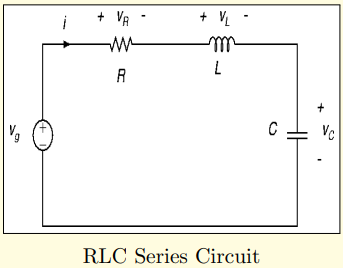
\includegraphics[width=0.50\textwidth]{i6.png}
    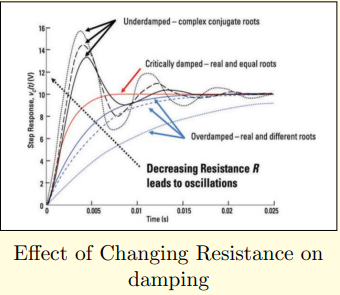
\includegraphics[width=0.45\textwidth]{i7.png}
\end{center}
\subsection{Breadboard}
\begin{center}
    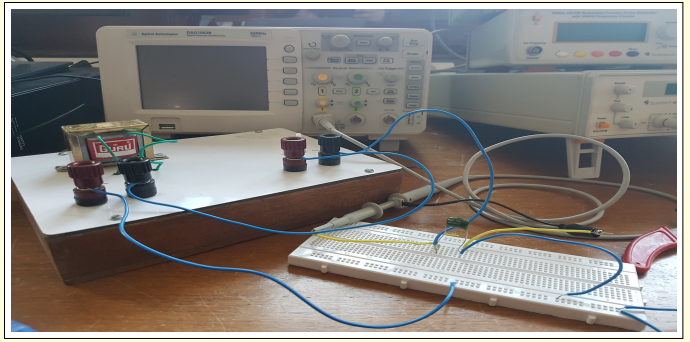
\includegraphics[width=0.8\textwidth]{i8.png}
\end{center}
\subsection{Observation}
\begin{center}
\begin{tabular}{|c|c|c|}
\hline
    Resistance($\Omega$) & $\alpha$ & $\omega_{0}$ \\
    \hline
    500 & 125 & 1507.55 \\
    5800 & 1450 & 1507.55 \\
    10000 & 2500 & 1507.55 \\
\hline
\end{tabular}
\end{center}

\subsection{Calculation}
For Critically Damped Case, $\alpha$ = $\omega_{0}$.\\
Thus, R=2L$\omega_{0}$. or R = 2 × 2 × 1507.55 = 6030.2$\Omega$

\subsection{Error Analysis}
Calculated Value of R for Critical Damping= 6.03 k$\Omega$ \\
Measured Value of R for Critical Damping= 5.80 k$\Omega$ \\
Thus, Error= 0.23 k$\Omega$ \\
Error Percentage= $\frac{0.23}{6.03}$× 100 = 3.8\%

\subsection{Time Domains}
\subsubsection{Under Damped Circuit}
\begin{enumerate}
    \item $\Delta$V = 4.32V (Step Voltage)
    \item $t_{d}$ = 800µs (Time till it reaches half the Step Voltage)
    \item $t_{r}$ = 1.16ms (Time till it reaches Step Voltage First time)
    \item $t_{p}$ = 2.12ms (Time till Overshoot Voltage)
    \item $t_{s}$ = 11.7ms (Time till deflection from step voltage is $\leqslant$ 2\%)
\end{enumerate}
\subsubsection{Critically Damped Circuit}
\begin{enumerate}
    \item $t_{d}$ = 1ms (Time till it reaches half the Step Voltage)
    \item $t_{r}$ = 2.4ms (Time till it reaches Step Voltage First time)
\end{enumerate}
\subsubsection{Over Damped Circuit}
\begin{enumerate}
    \item $t_{d}$ = 1.62ms (Time till it reaches half the Step Voltage)
    \item $t_{r}$ = 5.2ms (Time till it reaches Step Voltage First time)
\end{enumerate}
\begin{center}
    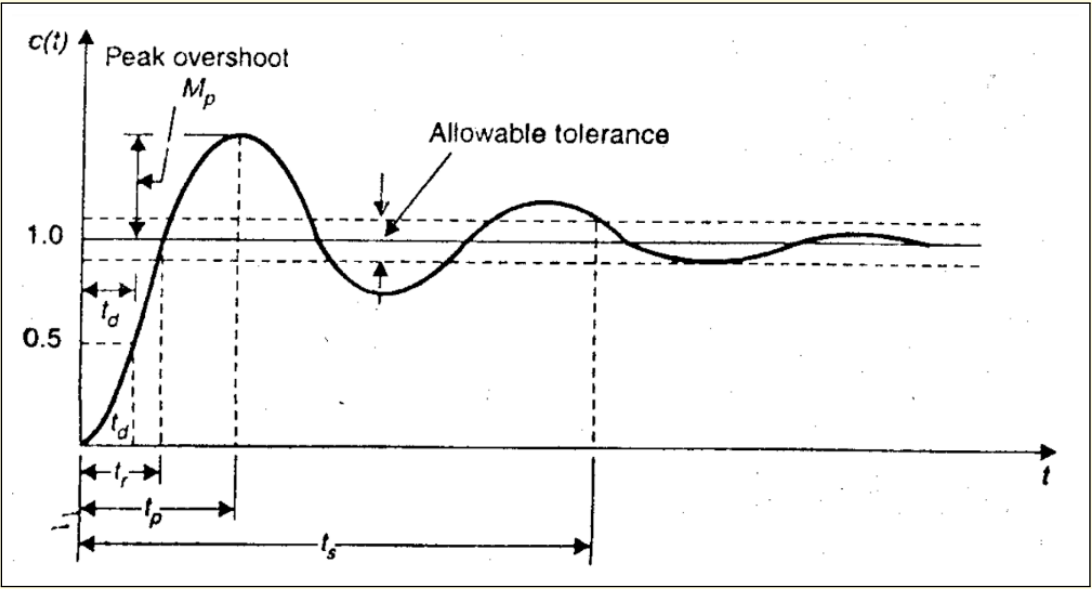
\includegraphics[width=0.8\textwidth]{i9.png}
\end{center}
\subsection{DSO Images}
    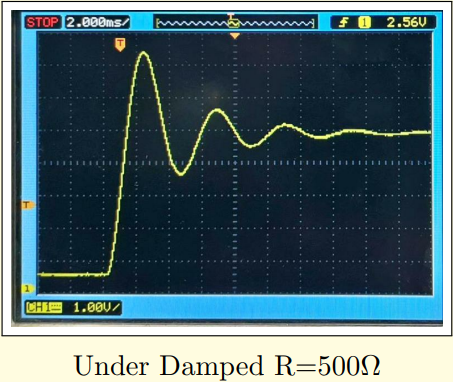
\includegraphics[width=0.5\textwidth]{i10.png}
    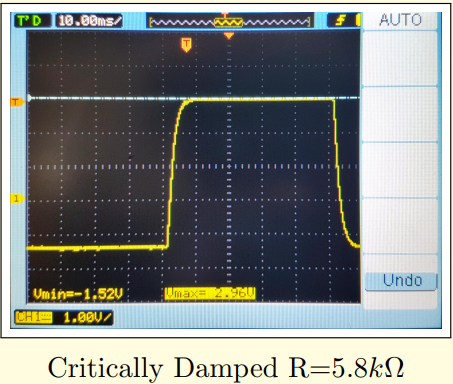
\includegraphics[width=0.5\textwidth]{i11.png}\\
    \\
    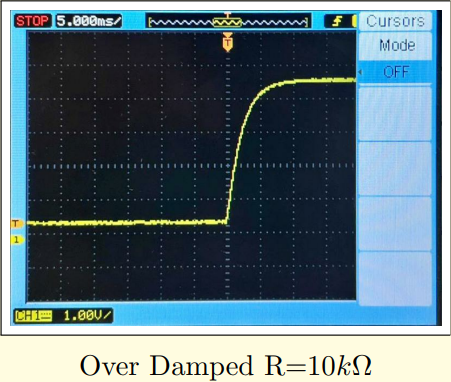
\includegraphics[width=0.55\textwidth]{i12.png}
    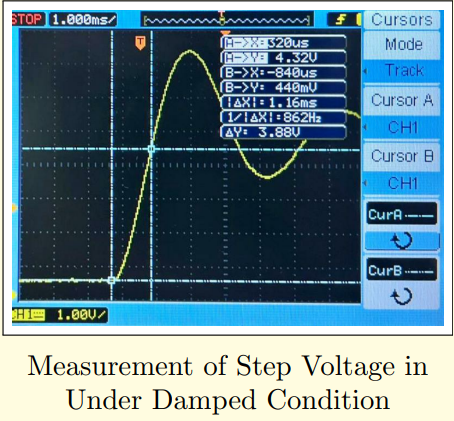
\includegraphics[width=0.5\textwidth]{i13.png}\\
    \\
    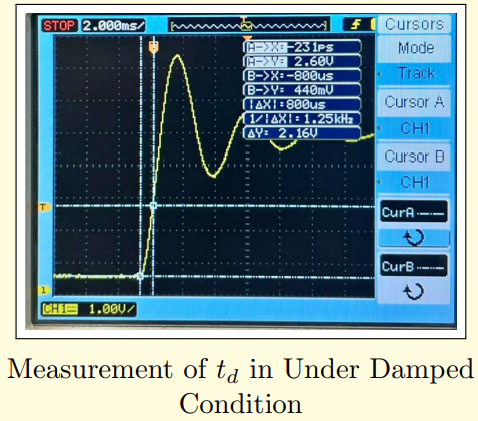
\includegraphics[width=0.52\textwidth]{i14.png}
    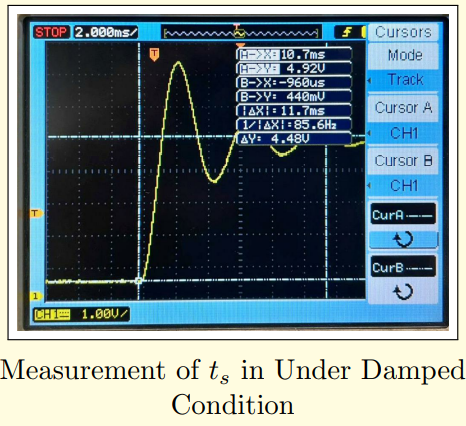
\includegraphics[width=0.5\textwidth]{i15.png}
\subsection{Conclusion}
Consequently, we were able to observe various damping conditions in the step response of a series RLC circuit and measure the various time domain specifications using a DSO device.
\newpage
\section{Sources of Error}
\begin{enumerate}
    \item Deviations due to tolerance in values.
    \item Resistance in wires and change due to temperature.
    \item Connections changed while circuit is powered.
    \item Loose connections.
    \item Difference in actual resistance, capacitance or inductance from measured value.
\end{enumerate}
\section{Precautions}
\begin{enumerate}
    \item Electric wires (jumpers) should be properly snipped.
    \item Circuit should not be left powered for long time.
    \item Proper shoes should be worn.
    \item Insulated tools should be used
\end{enumerate}
\section{Concluding Remarks}
In this experiment, the concept of step response in series RC and LCR circuits was demonstrated. In the initial phase of the experiment, the value of the time constant was derived from the graph displayed on the DSO screen. With a deflection of nearly 18.7 percent, the values were roughly equivalent to the theoretical values. This is within the experimental margin of error. In the second part of the experiment, we learned how to observe various types of damping in a series LCR circuit. In addition, we demonstrated that these cases are valid under under damped, over damped, and critically damped conditions. With a deflection of nearly 4 percent, we also confirmed that the resistance value for achieving a critically damped case came close to the theoretical value. Using the graphs obtained from the DSO display, we determined the various time domain specifications.
\end{document}
